\documentclass{article}


% Use documentclass{article}


\usepackage[english]{babel}
\usepackage[T1]{fontenc}
\usepackage{ragged2e}
\usepackage{amsfonts}
\usepackage{systeme}
\usepackage{amsmath}
\usepackage{amssymb}
\usepackage{comment}
\usepackage{multicol}
\usepackage{lipsum} 
\usepackage{graphicx}
\usepackage{stmaryrd}
\usepackage{systeme}
\usepackage{wrapfig}
\usepackage{colortbl}
\usepackage{cellspace}
\usepackage{stmaryrd}
\usepackage{ntheorem}
\usepackage{lmodern}
\usepackage{mathtools}
\usepackage{wrapfig}
\usepackage{ragged2e}
\usepackage{tabularx}
\usepackage{titlepic}
\usepackage{fancyhdr}
\usepackage{caption}
\usepackage{xcolor} % pour les couleurs
\usepackage[linkbordercolor=white]{hyperref} % après avoir chargé xcolor
\usepackage{systeme}
\usepackage[T1]{fontenc}
\usepackage{lmodern}
\usepackage{listings}
\usepackage{tikz}
\usepackage{mdframed}
\usepackage{xparse} % Nécessaire pour définir des environnements avec arguments optionnels
\usepackage[top=3cm, bottom=3cm, left=3.5cm, right=3.5cm]{geometry}

% \setcounter{secnumdepth}{-1} % Désactive le compteur des parties

% PAGE SETTINGS

% \justifying

% \setlength{\columnseprule}{1pt}
% \def\columnseprulecolor{\color{black}}

\newcolumntype{C}{>{$\displaystyle}Sc<$}
\cellspacetoplimit=5pt
\cellspacebottomlimit=5pt


% MATHS SHORTHANDS

\newcommand{\C}{\mathbb{C}}
\newcommand{\R}{\mathbb{R}}
\newcommand{\Q}{\mathbb{Q}}
\newcommand{\Z}{\mathbb{Z}}
\newcommand{\N}{\mathbb{N}}
\newcommand{\U}{\mathbb{U}}
\newcommand{\K}{\mathbb{K}}
\newcommand{\M}{\mathcal{M}}
\newcommand{\B}{\mathcal{B}}

\renewcommand{\epsilon}{\varepsilon}
\renewcommand{\phi}{\varphi}
\renewcommand{\rho}{\varrho}

% MOD NOTATION

\theorembodyfont{\upshape}

% Définir un environnement pour encadrer les définitions avec un titre
\NewDocumentEnvironment{definition}{O{}}
{
  \begin{mdframed}[linewidth=0pt,linecolor=gray,backgroundcolor=gray!10,roundcorner=5pt]
  \textbf{Définition}%
  \IfNoValueTF{#1}{}{~(\textbf{#1})} % Affiche le titre entre parenthèses et en gras s'il est fourni
  . % Point à la fin
}
{
  \end{mdframed}
}

% Définir un environnement pour encadrer les théorèmes avec un titre
\NewDocumentEnvironment{theorem}{O{}}
{
  \begin{mdframed}[linewidth=1pt,linecolor=darkgray,backgroundcolor=darkgray!10,roundcorner=5pt]
  \textbf{Théorème}%
  \IfNoValueTF{#1}{}{~(\textbf{#1})} % Affiche le titre entre parenthèses et en gras s'il est fourni
  . % Point à la fin
}
{
  \end{mdframed}
}

% Définir un environnement pour encadrer les corollaires
\NewDocumentEnvironment{corollary}{O{}}
{
  \begin{mdframed}[linewidth=1pt,linecolor=gray,backgroundcolor=gray!10,roundcorner=5pt]
  \textbf{Corollaire}%
  \IfNoValueTF{#1}{}{~(\textbf{#1})} % Affiche le titre entre parenthèses et en gras s'il est fourni
  . % Point à la fin
}
{
  \end{mdframed}
}
				

\theoremstyle{plain}
\newtheorem*{remark}{Remarque}
\newtheorem*{proposition}{Proposition}
\newtheorem*{lemma}{Lemme}
\newtheorem*{prop}{Propriété}
\newtheorem*{proof}{Démonstration}
\newtheorem*{example}{Exemple}


% OTHERS 


%\newlength\tindent
%\setlength{\tindent}{\parindent}
%\setlength{\parindent}{0pt}
%\renewcommand{\indent}{\hspace*{\tindent}}

% Put begin and end document 

\usepackage[utf8]{inputenc}


\begin{document}


% ==================================================================================================================================


\begin{center}
    \textbf{ - Projet Réseau - }

    \Large{\textbf{Hermes}}
\end{center}

\rule{\linewidth}{1.5pt}


% ==================================================================================================================================

\justify

\subsection{Introduction}

Ici, est présenté le Projet \texttt{Hermes} dans les grandes lignes. Nous allons aborder différents aspects du projet. 
Celui-ci se décompose en deux parties. Une première version, disons bêta \texttt{Chatty}, étant simplement un chat sécurisé entre deux utilisateurs. 
La seconde version, disons finale \texttt{Hermes}, un client de chat en ligne sécurisé multi-threadé. 

Nous allons d'abord commencer par présenter Chatty, puis nous parlerons en détail d'Hermes. 
Dans cette seconde partie nous aborderons des notions de cryptographie pour expliquer en détail quels procédés les différentes 
intances de Hermes utilisent pour chiffrer les messages. Une explication de la fonction de chaque fichier sera donné dans les grandes lignes. 
Pour finir, nous évoquerons les failles de sécurité présentes dans le projet, les éventuelles améliorations possibles. 
Nous finirons par un court tutoriel permettant de tester toutes le fonctionnalités d'Hermes. 

\vspace{0.5cm}

Bonne lecture !

\section{Structure du projet - Diagramme de classes}

\begin{figure}[h]
    \centering
    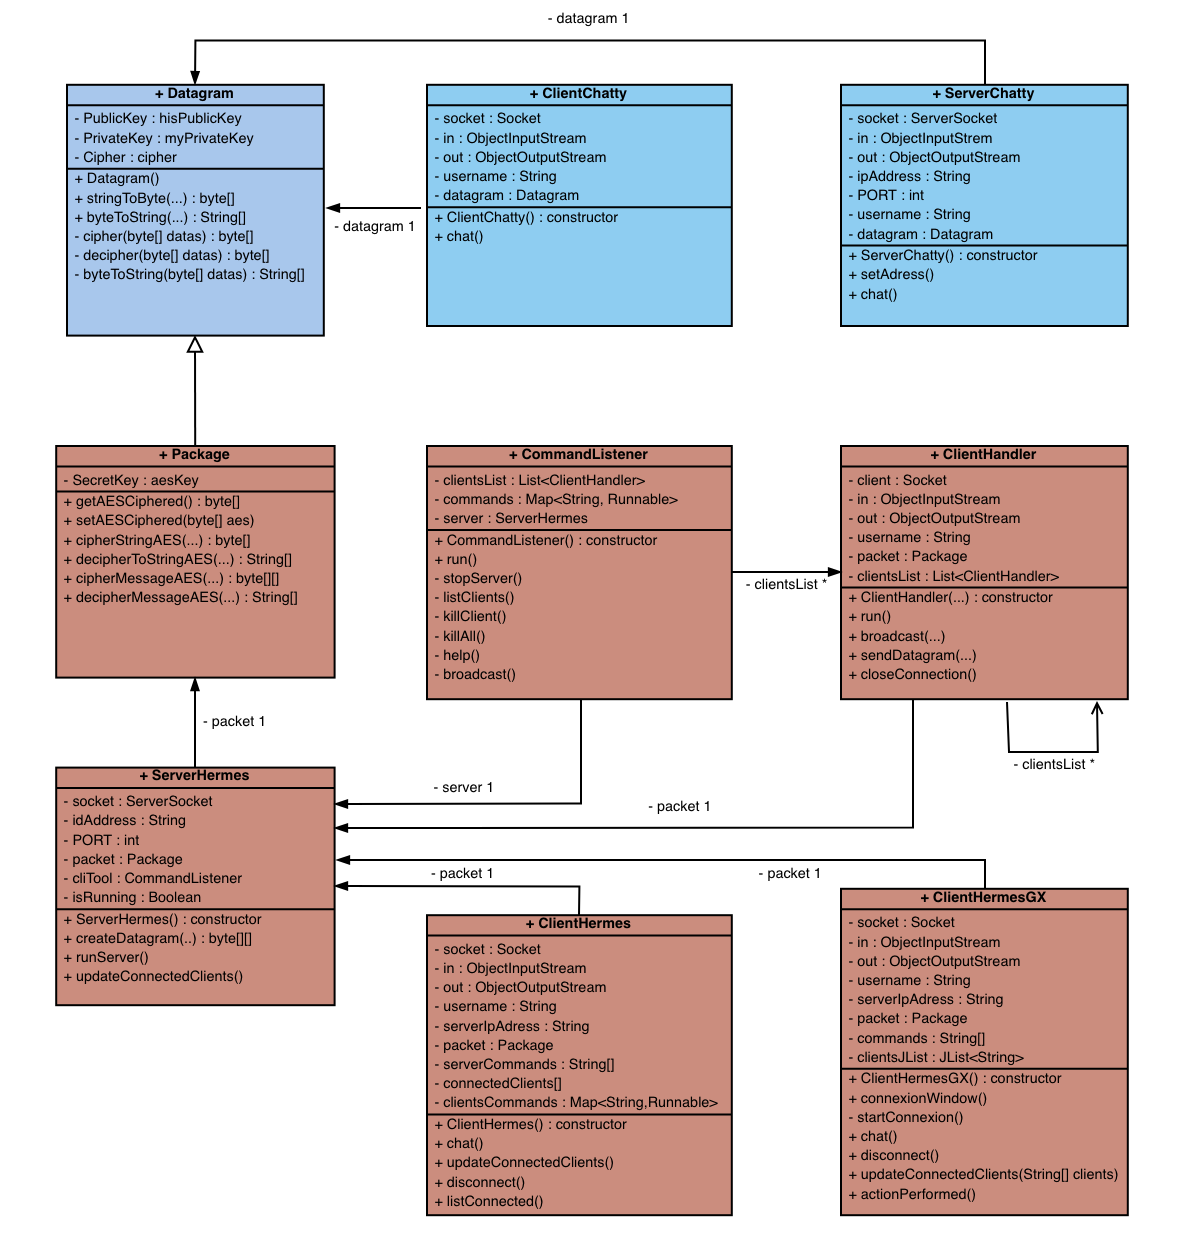
\includegraphics[width=0.7\textwidth]{class_diagramm.png}
    \caption{Diagramme de classes du projet}
    % \label{fig:example}
\end{figure}

\section{Chatty}

\subsection{Principe}

Chatty est une application de chat en ligne de commande permettant à deux utilisateurs de discuter en toute sécurité grâce au protocole RSA. 

Un utilisateur se connecte en tant que serveur, l'autre en tant que client. 
Le serveur doit physiquement donner son adresse IP au client et le client doit la rentrer dans le logiciel pour 
permettre la connexion. Ici, on utilise des sockets pour établir une connexion. La connexion par socket n'étant pas chiffré, 
on utilise un système de chiffrement RSA pour, d'une part permettre l'échange des clés en toute sécurité, et d'autre part, 
une communication sécurisée. 

Comparé à Hermes, vu ci-dessous, Chatty n'utilise pas AES puisque c'est une version bêta d'Hermes. 

\subsection{Fonctionnement Général}

Pour permettre l'échange de messages entre deux utilisateurs, le premier doit donc lancer \texttt{ServerChatty} et l'autre 
\texttt{ClientChatty}. Comme dans Hermes plus bas, le client se connecte via un Socker au serveur, sauf qu'ici, pas de 
multi-threading, les deux programmes s'échangent directement les clés RSA, puis AES et discuttent entre eux. 
On utilise le même Socket pour les deux utilisateurs, lors des tests, aucuns problème n'a été observé. 
On peut utiliser la commande \texttt{exit} pour arrêter proprement le programme. 

\newpage

\section{Hermes}

\subsection{Principe}

Ici, on attaque des choses un peu plus compliquées. 
Un serveur accepte des connexion socket de clients et s'occupe de router les messages reçus vers les destinataires désignés. 
On utilise des Threads pour permettre d'écouter et de gérer chaque client connecté séparément. 


\subsection{La structure des messages - Classe \texttt{Package}}

Comme pour Chatty, on utilise une classe spéciale pour gérer le chiffrement/déchiffrement des messages à envoyer via le socket.
Ici, \texttt{Package} qui hérite de \texttt{Datagram}. Elle implémente de nouvelles méthodes, telles que le chiffrement/déchiffrement AES. 

Cela permet, d'une part de factoriser le code côté server et client et d'autre part, de rajouter une couche d'abstraction. 
Les attributs de la classe \texttt{Package} sont majoritairement privés, permettant une meilleure sécurité. 

\subsubsection{Gestionnaire AES}

On souhaite pouvoir échanger des messages via socket sans craindre de se faire observer. On va donc chiffrer tous les flux 
traversant le socket via un algorithme de chiffrement, ici AES. 
C'est un algorithme de chiffrement dit symétrique (même clé pour le chiffrement et déchiffrement). 
On utilise principalement 4 méthodes pour permettre le chiffrement/déchiffrement avec AES : 
\begin{itemize}
    \item \texttt{cipherStringAES()} : Permet simplement le chiffrement d'une chaîne de caractère avec AES. 
    On l'utilise pour envoyer le nom d'utilisateur du client au serveur à l'initialisation de connexion (utile pour le routage des paquets). 
    \item \texttt{decipherToStringAES()} : L'inverse de la méthode précédente, elle déchiffre des tableaux de bits (\texttt{byte[]}) 
    avec AES. Elle sert lors de la réception du nom d'utilisateur lors de l'initialisation de la connexion.
    On s'en sert aussi lors du routage des paquets pour déchiffrer le nom d'utilisateur de l'envoyer et du destinataire. 
    \item \texttt{cipherMessageAES()} : Côté client, elle permet de créer un paquet contenant date et heure d'envoi, utilisateur 
    envoyeur du paquet, destinataire et message envoyé. Le tout méticuleusement chiffré avec une clé AES de 256 bits. 
    \item \texttt{decipherMessageAES()} : coté client récepteur d'un paquet, elle extrait toutes les informations de celui-ci pour 
    permettre leur traitement par le client après l'avoir déchiffré. 
\end{itemize}

Le problème est que, malgré la force d'AES, sa rapidité d'exécution et sa fiabilité, cela reste un algorithme de chiffrement symétrique. 
Il faut donc que les deux parties s'échangent la clé à l'initialisation de la connexion pour permettre l'échange de messages chiffrés. 
Il est bien évidement inenvisageable d'envoyer la clé AES en clair sur le réseau, la rendant visible pour toute personne écoutant le flux de paquets. 
On utilise pour cela RSA...

\subsubsection{Gestionnaire RSA}

Tout comme AES, la classe \texttt{Package}, permet aux classes l'utilisant de chiffrer/déchiffrer avec l'algorithme RSA. 
RSA est un algorithme de chiffrement asymétrique paru en 1977. Une clé (dite publique) sert à chiffrer les messages et une autre (dite privée) à les déchiffrer. 
La force de cet algorithme est le fait que l'on ne peut retrouver la clé privée à partir de la clé publique en temps raisonnable. 

On va donc se servir de RSA pour partager la clé AES entre le serveur et le client et ainsi permettre un échange de paquets en toute sécurité. 

Ainsi, à l'initialisation de la connexion, le client, qui a généré des clés RSA à son instanciation envoie sa clé publique 
au serveur pour que celui-ci lui renvoie la clé AES chiffrée en RSA qu'il utilise pour communiquer avec chaque client. 
Le client reçoit alors un paquet constitué d'une séquence de bits apparement illisibles mais qu'il peut déchiffrer en une parfaite 
clé AES pour ensuite envoyer des messages chiffrés avec celle-ci. 

La classe \texttt{Package} permet différentes deux utilisations de l'algorithme RSA au travers de deux méthodes :
\begin{itemize}
    \item \texttt{getAESCiphered()} : Utilisée côté serveur, elle sert à chiffrer la clé AES générale avec la clé publique RSA 
    du client pour la lui envoyer en toute sécurité. 
    \item \texttt{setAESCiphered()} : Côté client, elle déchiffre le paquet reçu par le serveur chiffré en RSA pour récupérer la clé AES 
    et la rajouter à son trousseau. La discussion peut ensuite commencer entre le serveur et le client sans que personne ne puisse savoir ce qu'il se disent.
\end{itemize}

On choisit volontairement d'utiliser deux méthodes de chiffrement pour une simple raison. 
RSA étant très puissant, il est malgré tout très lent comparé à AES du fait qu'il utilise un algorithme assez complexe. 
AES, quand à lui, est basé sur DES, algorithme effectuant seulement des permutations et xor de bits. 
Ainsi, pour chiffrer un gros volume de bits et permettre l'envoi de long messages rapidement, sans trop de délai, AES est une option de choix. 
On utilise donc RSA seulement pour envoyer la clé AES au début de la connexion. 


\subsubsection{Structure d'un paquet}

Les paquets envoyés dans le Socket par les client sont seulement des matrices de bits dont chaque ligne correspond à une information :
\begin{itemize}
    \item Les destinataire du paquet pour savoir, côté serveur, à qui faire parvenir le paquet. 
    \item La personne ayant envoyé le paquet, pour éviter de lui renvoyer le paquet en cas de broadcast. 
    \item Le message envoyé ainsi que la date et l'heure de l'envoi. 
\end{itemize}
Le tout, bien entendu, chiffré avec AES. 

\subsection{Le serveur - Classe \texttt{ServerHermes}}

La classe \texttt{ServerHermes} constitue le coeur même du serveur. 
Elle permet deux choses :
\begin{itemize}
    \item \textbf{Initialiser le Socket : } à son lancement, elle ouvre un socket sur un port déterminé et génère les outils 
    de sécurité nécessaires au bon fonctionnement d'\emph{Hermes}. 
    \item \textbf{Accepter les connexions : } Un Thread permet d'accepter en continu les connexions de clients (classes \texttt{ClientHermes}). 
    Une fois un client accepté, la méthode \texttt{runServer()} créé un nouveau \texttt{ClientHandler} pour gérer séparément 
    la connexion avec le nouveau client connecté. 
\end{itemize}

\subsection{Le gestionnaire de clients - Classe \texttt{ClientHandler}}

La classe \texttt{ClientHandler} permet de gérer indépendamment chaque client connecté au Server via un Thread. 
Lorsque le serveur accepte un nouveau client, il délègue toute sa gestion à \texttt{ClientHandler}. 

Ainsi, cette classe s'occupe d'instancier les entrées/sorties pour le Socket et d'échanger les clés RSA/AES. 
Un Thread \texttt{run()} permet de récupérer les messages reçu par le client et, via la liste des clients connectés, 
de renvoyer les messages au bon correspondant. 

Des méthodes \texttt{broadcast()} et \texttt{disconnect()} permettent une meilleure gestion du client. 


\subsection{Le client - Classe \texttt{ClientHermes}}

Cette classe permet à n'importe quelle machine de se connecter au Server Hermes via une interface en ligne de commande. 
Comme vu précédement, une fois le nom d'utilisateur choisit et saisit, la classe s'occupe de se connecter au server en échangeant 
les clés RSA pour ensuite se faire envoyer la clé privée AES. 
Une fois cela fait dans le constructeur, une méthode \texttt{chat()} permet, d'un côté d'écouter l'entrée sur le socket via un Thread
pour récuprérer les messages entrants. Et de l'autre, d'écouter l'entrée utilisateur pour ensuite envoyer les messages dans le Socket. 

\subsection{Le client (version graphique) - Classe \texttt{ClientHermesGX}}

Malgré le fait que la classe \texttt{ClientHermes} en ligne de commande soit assez conviviale, pour les allergiques à un terminal
il existe une version graphique du client Hermes. 
Cela se passe de la même façon que pour le client en ligne de commande, une première fenêtre s'ouvre pour saisir l'adresse ip du serveur 
(localhost par défaut) et le nom d'utilisateur. Une fois le boutton \texttt{Connect} pressé, la méthode \texttt{startCOnnexion()} initialise 
la connexion au server via un socket de façon sécurisée (voir 2.2.1 et 2.2.2). 
Une fenêtre décomposée en trois panneaux permet d'un côté, d'afficher les clients connectés au serveur, d'afficher l'historique des messages envoyés et reçus
et d'envoyer des messages. 

La méthode \texttt{updateConnectedClients()} permet de mettre à jour la liste des clients connectés et donc le panneau correspondant dès la réception d'un 
packet commande par le serveur. 

\newpage

\section{Petits trucs en plus...}

Vous l'aurez sûrement remarqué, Tou n'est pas abordé dans ce rapport. Du moins, pas encore... 
En effet, pas mal de fonctionnalités on été ajoutées pour, d'un côté, améliorer l'expérience utilisateur, mais aussi permettre une meilleure sécurité. 

\subsection{Une interface pour le serveur ?}

Lorsqu'on lance le serveur, on voudrais dans l'idéal savoir qui est connecté, pouvoir envoyer des messages à tout le monde et déconnecter des clients 
un peu trop embêtant. C'est possible grâce à la classe \texttt{CommandListener}, un petit gestionnaire de ligne de commande pour le serveur. 
L'invite de commande se présente sous la forme suivante : \texttt{Hermes-Server:/\$} et permet plusieurs choses :
\begin{itemize}
    \item \texttt{/help} : liste les commandes possibles 
    \item \texttt{/stop} : déconnecte tous les clients et stope le serveur 
    \item \texttt{/killOne} : déconnecte un client 
    \item \texttt{/killAll} : déconnecte tous les clients 
    \item \texttt{/broadcast} : envoie un message à tous les clients 
\end{itemize}

Ainsi, dans \texttt{ClientHermes} et \texttt{ClientHermesGX}, on définit des tableaux correspondant aux commandes que le serveur 
peut envoyer. Lors de la lecture d'un message entrant dans le socket, on vérifie si ce n'est pas une commande provenant du serveur avant de l'afficher.
D'autres types de commandes existent, telles que celles permettant le listing des clients connectés et la déconnexion côté client en ligne de commande. 
On définit aussi une autre commande venant du serveur, côté client, permettant la mise à jour de la liste des clients connectés. 

\subsection{Fenêtre d'erreur}

Une fenêtre d'erreur pour l'interface graphique a été mise en place pour rapidement et efficacement avertir l'utilisateur 
de tout dysfonctionnement du logiciel. 

\subsection{Envoi de commandes - côté serveur}

On permet aussi au serveur d'envoyer des packet "commande" au clients. 
Cela est utile pour, par exemple, déconnecter un client (ex : commande \texttt{/killOne} et commande \texttt{/killAll} de \texttt{CommandListener}),
ou d'envoyer la liste des clients connectés. 

Une fois encore, lors de la lecture du message entrant dans le socket côté client, on vérifie si c'est un packet "commande" 
avant l'affichange dans la ligne de commande ou la fenêtre. 


\subsection{Commandes côté client - Classe \texttt{ClientHermes}}

Dans \texttt{ClientHermes} on permet à l'utilisateur de saisir des commandes, permettant deux choses :
\begin{itemize}
    \item \texttt{/listConnected} : liste les autres personnes connectés à Hermes. 
    \item \texttt{/disconnect} : pour fermer proprement la connexion à Hermes. 
\end{itemize}


\section{Limites et améliorations possibles}

Malgré la grosse quantité d'heures de travail apportées au projet, il reste quand même beaucoup de choses à améliorer, et de failles de sécurité potentielles. 

\subsection{Un client malin}

Lors du lancement d'un client Hermes, un petit malin peut facilement s'attribuer beaucoup de pouvoir. 
En effet, si l'on regarde bien le code côté client, lors de la réception d'un paquet commande, on vérifie
que le champs de message contient bien une commande et que la personne émettrice est bien le serveur. 
Problème, on identifie le serveur via son username ("Server") et non une clé d'authentification AES/GPG. 
Un client un peu malin peut donc, lors de sa connexion, saisir comme username "Server" et envoyer des messages commandes 
dans le général. Normalement, les autres clients interprèterons les messages comme des commandes venant du serveur. 

\vspace{0.5cm}

Patchs possibles : 
\begin{itemize}
    \item Premièrement, \textbf{empêcher la connexion d'un client avec le username "Server"}, assez compliqué 
    à faire, il faudrait que le client soit en capacité de gérer un refus de connexion. Il est bien sûr inenvisageable de simplement 
    vérifier le username côté client... 
        \begin{center}
            \textbf{Règle n°1 : Ne jamais faire confiance au client.}
        \end{center}
    \item Une autre façon de faire, plus simple, \textbf{vérifier lors du routage des paquets}, côté serveur qu'aucun paquet ne circule avec le 
    username "Server", si on en trouve un, ne pas le router et lancer un \texttt{/killOne} sur l'utilisateur émetteur.
\end{itemize}

\subsection{Une clé pas très secrète}

Admettons que vous voulez écouter tout ce qui se dit sur Hermes. Vous avez juste, soit à récupérer le code du client ou à 
facilement retrouver comment s'y connecter avec un peu de motivation. 
Une fois cela fait, vous arrivez à vous connecter à Hermes et récupérez donc l'unique clé AES permettant le chiffrement de tous les 
messages. La dite clé n'étant regénérée que lorsque le serveur est éteint, si il tourne longtemps, tout client qui s'est connecté au moins 
une fois a en sa possession la clé AES permettant aux client connectés de discuter en sécurité. 
On peut considérer cela comme un soucis...

\vspace{0.5cm}

Patch possibles : 
\begin{itemize}
    \item \textbf{Dès qu'un client se déconnecte, mettre à jour la clé AES.} C'est à dire, en regénérer une et l'envoyer à tout le monde 
    pour ne pas que le client précédement connecté puisse écouter les messages échangés. Cela s'implémenterai assez simplement 
    étant donné que l'on met déjà à jour la liste des clients connectés à chaque connexion/déconnexion. On pourait simplement envoyer 
    la nouvelle clé AES en plus. 

    Cependant, cette nouvelle clé AES pourrait elle-aussi être déchiffrée par le client déconnecté. Pour cela, c'est plutôt les clés RSA 
    qu'il faudrair changer. Bref....un beau bordel... 
    \item \textbf{Avoir une clé AES différente pour chaque client connecté.} Plus fiable pour les connexions/déconnexions de clients. 
    Mais cela pose un vrai problème de sécurité côté serveur. En effet, pour chaque message à router, le serveur devrait le déchiffrer 
    avec la clé AES du client émetteur et le chiffrer avec les clés AES des clients destinataires. Problème : à un moment donné, 
    tout le contenu du message serait stocké en clair dans une variable du serveur. Pour un attaquant étant connecté physiquement au serveur 
    ou ayant accès à ses registres, il pourrait voir tous les messages échangés. 
\end{itemize}

\subsection{Améliorations}

Ainsi, on peut envisager plusieurs améliorations :
\begin{itemize}
    \item \textbf{Pouvoir sélectionner le destinataire du message} (côté client).
    La structure d'Hermes le permet déjà, il faut simplement modifier le champs destinataire lors de la construction du 
    paquet côté client. Le serveur s'occupe déjà de bien router les paquets en fonction de ce champ. 
    \item \textbf{Faire en sorte que le serveur soit incapable de déchiffrer les messages envoyés.} 
    Pour cela, chaque couple de clients possède un clé AES secrète permettant de s'échanger les messages. 
    Cela semble assez compliqué à implémenter... 
    \item \textbf{Améliorer l'interface graphique.} 
    Lors des tests vous verrez bien que l'interface graphique n'est pas au top... 
\end{itemize}


\section{Tests et Guide d'utilisateur}

\subsection{Instructions de test}

Pour que le guide de test suivant fonctionne bien, il est préférable d'utiliser un machine Linux/MacOS. 
Si ce n'est pas possible, il faudra modifier le Makefile en fonction du système d'exploitation.
Le plus pratique est de directement cloner le repo Github à l'adresse suivante :
\begin{center}
    \href{https://github.com/winston2968/Hermes.git}{https://github.com/winston2968/Hermes.git}
\end{center}

Une fois cela fait, vérifiez que la commande \texttt{make} est bien installée. Ensuite, vous pouvez exécuter les commandes 
suivantes pour la compilation et l'exécution des différentes classes du projet. Veillez à bien rester dans le dossier \texttt{Hermes/}
pour l'exécution des commandes. 
\begin{itemize}
    \item \texttt{make clean \&\& make compile} : nettoie le dossier \texttt{/bin} et compile toutes les classes .java dans ce dossier. 
    \item \texttt{make run-hermes-server} : lance le serveur Hermes 
    \item \texttt{make run-hermes-client} : lance le client en ligne de commande 
    \item \texttt{make run-hermes-clientGX} : lance le client hermes en interface graphique 
    \item \texttt{make run-chatty-server} : lance le serveur chatty 
    \item \texttt{make run-chatty-client} : lance le client chatty 
\end{itemize}

Durant le développement d'Hermes, il était important de pouvoir lancer plusieurs fois le même fichier de code, 
comme les clients Hermes, pour vérifier que le multi-threading fonctionnait bien. Pour cela, après quelques recherche,
le plus simple était de directement compiler/lancer les fichier depuis le terminal. Ainsi, le recours à un Makefile pour 
factoriser les commandes semblait indispensable. 

\begin{quote}
    Pour plus d'informations, le descriptif des commandes est donné dans le fichier \texttt{Makefile}.
\end{quote}


\end{document}
